
\section{Importing the Empty Project from GitHub}

The following instruction to guide you create a Maven Git project is similar to
a blog
post\footnote{\url{http://springinpractice.com/2012/05/06/mavenizing-an-empty-github-project-in-eclipse/}}.
In fact, you could create a Maven Git project in various ways. For example, you
can create a Maven project first, and share it to Git, or you can just create a
Java project, and add Maven nature, then share it to Git, and so on. But, we
will show you the way that we think the most comfortable to achieve the goal.

\subsection{Checking out the empty GitHub project}

\begin{enumerate}

\begin{figure}[t]
\hspace{-2em}
\begin{minipage}{0.5\textwidth}
\centering
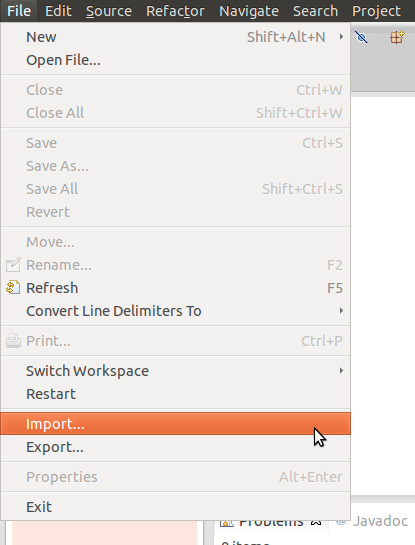
\includegraphics[scale=0.3]{project-01-import}
\caption{Importing project hosted on GitHub\label{project-01-import}}
\end{minipage}
\hfill
\begin{minipage}{0.5\textwidth}
\centering
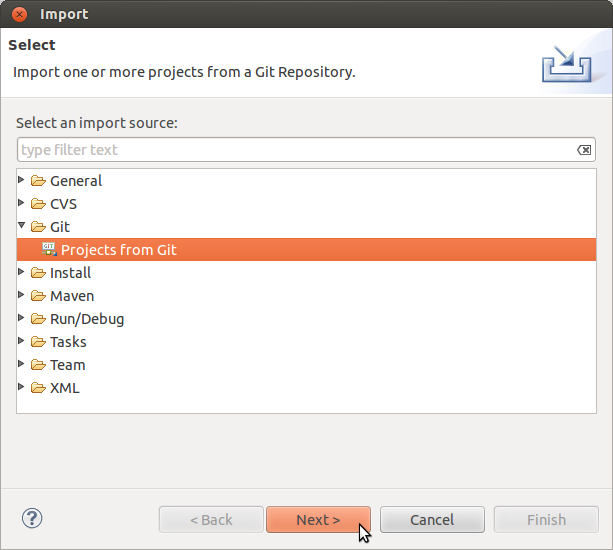
\includegraphics[scale=0.3]{project-02-git}
\caption{Choosing Git project\label{project-02-git}}
\end{minipage}
\hspace{-2em}
\end{figure}

\item Click \textbf{File} $\rightarrow$ \textbf{Import\ldots} to get ready to
import the empty project hosted on GitHub to local filesystem, as shown in
Figure \ref{project-01-import}.

\item Then select \textbf{Git} $\rightarrow$ \textbf{Projects from Git} in the
\textbf{Import} window. See Figure \ref{project-02-git}.

\begin{figure}[t]
\hspace{-2em}
\begin{minipage}{0.5\textwidth}
\centering
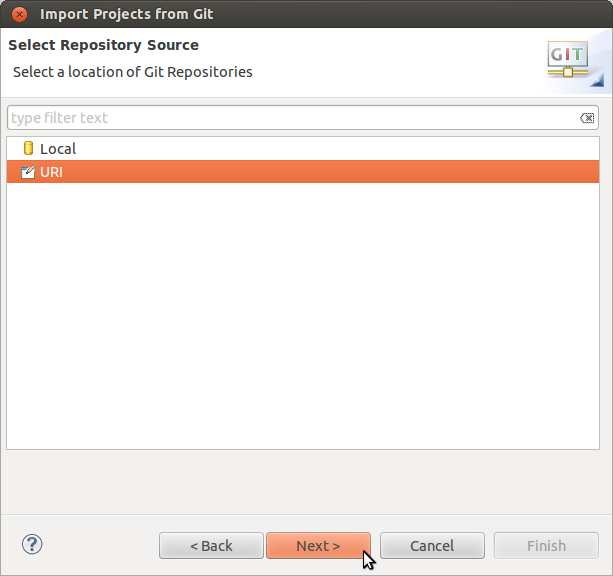
\includegraphics[scale=0.3]{project-03-git-uri}
\caption{Choosing to import Git project specified by a URI\label{project-03-git-uri}}
\end{minipage}
\hfill
\begin{minipage}{0.5\textwidth}
\centering
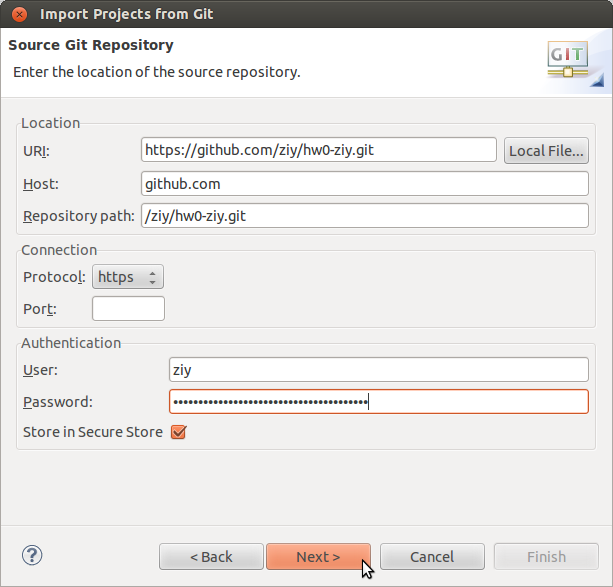
\includegraphics[scale=0.3]{project-04-git-repo}
\caption{Typing in your GitHub repository URI\label{project-04-git-repo}}
\end{minipage}
\hspace{-2em}
\end{figure}

\item Select \textbf{URI} as the repository source, then click \textbf{Next}.
See Figure \ref{project-03-git-uri}.

\item Copy the URI from your GitHub repository page (c.f. Figure
\ref{git-03-uri}), and paste it here as the URI, and the Host and Repository
path will be automatically generated for you. You also need to type in your Git
Repository username and password, and probably you want to \textbf{Store in in
Secure Store}. So just check the box at the bottom of the window, and then click
\textbf{Next}. See Figure \ref{project-04-git-repo}.

\begin{figure}[t]
\hspace{-2em}
\begin{minipage}{0.5\textwidth}
\centering
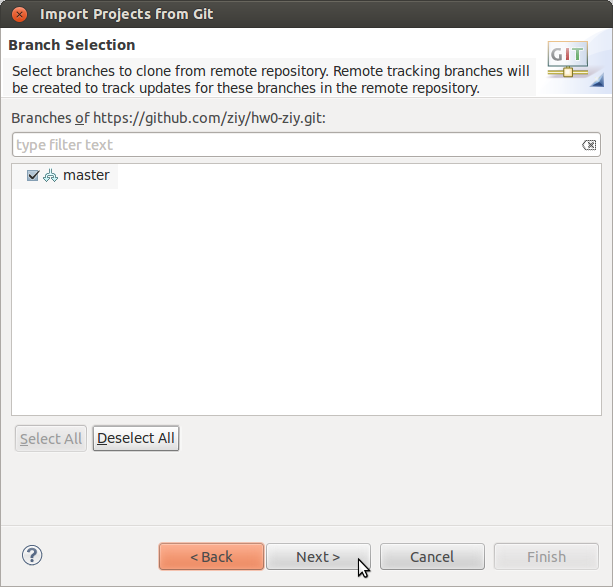
\includegraphics[scale=0.3]{project-05a-git-empty}
\caption{Choosing master branch\label{project-05a-git-empty}}
\end{minipage}
\hfill
\begin{minipage}{0.5\textwidth}
\centering
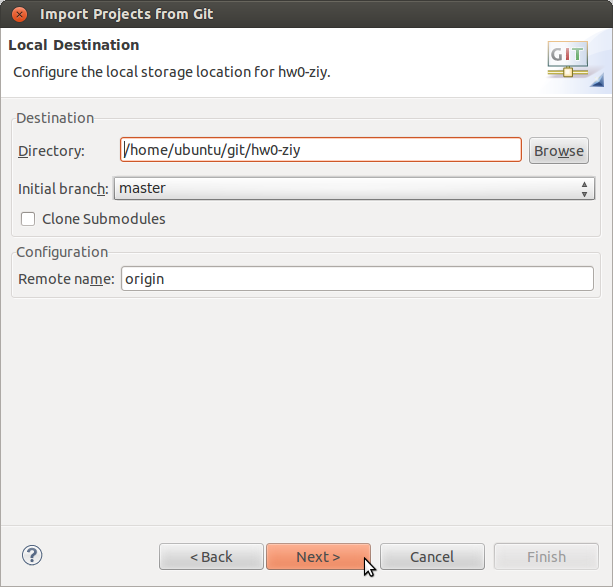
\includegraphics[scale=0.3]{project-06a-git-local}
\caption{Choosing local Git project location\label{project-06a-git-local}}
\end{minipage}
\hspace{-2em}
\end{figure}

\item Most of the time, you will see EGit plug-in is able to detect the branch
\textbf{master} does exist in the repository (as shown in Figure
\ref{project-05a-git-empty}). Click \textbf{Next} to proceed to the next step
where you can specificy the local storage location for the project. If you are
not sure what it means by a local storage, you should go back to Task 1 to learn
one of the most important features of Git - distributed version control. Type in
your local storage path in \textbf{Directory}, and \textbf{master} will be
selected by default as the \textbf{Initial branch} as shown in Figure
\ref{project-06a-git-local}. Now you could proceed to next step.

\begin{figure}[t]
\hspace{-2em}
\begin{minipage}{0.5\textwidth}
\centering
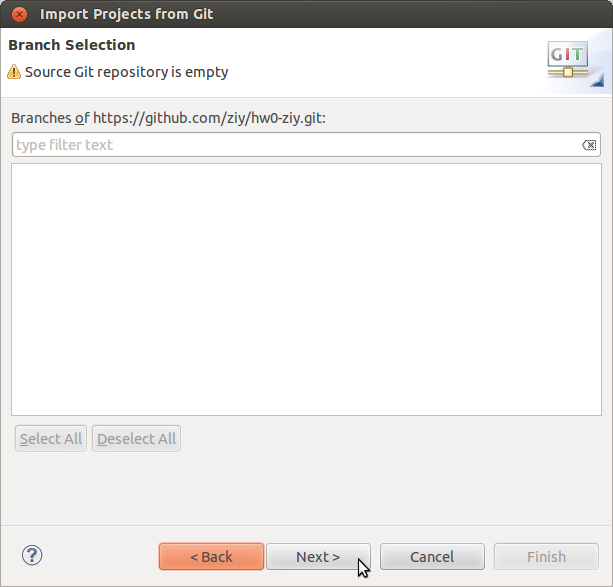
\includegraphics[scale=0.3]{project-05-git-empty}
\caption{Failed to choose master branch\label{project-05-git-empty}}
\end{minipage}
\hfill
\begin{minipage}{0.5\textwidth}
\centering
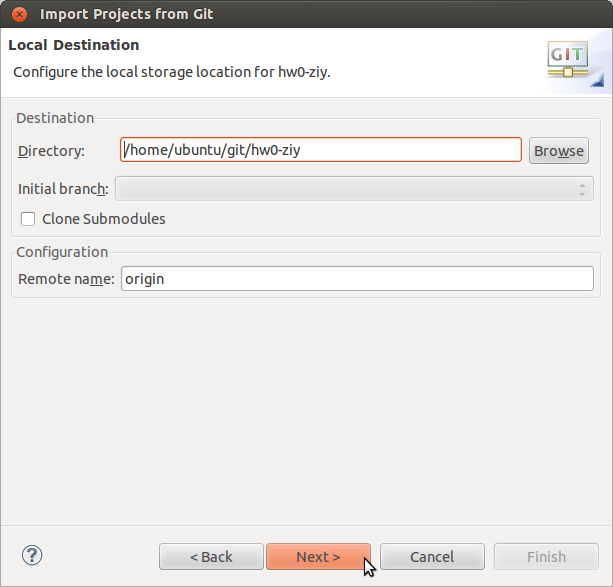
\includegraphics[scale=0.3]{project-06-git-local}
\caption{Choosing local Git storage location for the project\label{project-06-git-local}}
\end{minipage}
\hspace{-2em}
\end{figure}

\begin{qa}

\item[Q1] If the master branch cannot be found automatically by EGit, i.e.,
Figure \ref{project-05-git-empty} is shown, where it says \textbf{Source Git
repository is empty} and no branch can be selected, instead of Figure
\ref{project-05a-git-empty}. What should I do?

\item[A1] No problem. You could still click \textbf{Next} to proceed, and in the
next window, you can still assign a local storage for the project, but you
cannot specify the \textbf{Initial branch} (see Figure
\ref{project-06-git-local}). You can specify the master branch at a later stage
when we try to perform your first git-commit.

\end{qa}

\item Finally, if you chose to store the password in a secure store, you need to
type in (of course twice) a master password for the secure storage. Note that
this is not your Maven or GitHub password, and it is only used within the scope
of Eclipse. See Figure \ref{project-07-git-password}.

\begin{figure}[t]
\centering
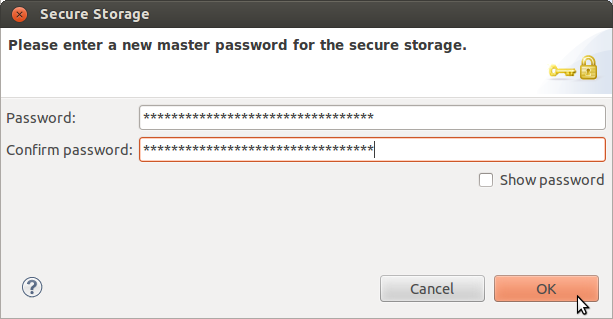
\includegraphics[scale=0.3]{project-07-git-password}
\caption{Typing in your password\label{project-07-git-password}}
\end{figure}

\end{enumerate}

\subsection{Creating a Maven project}

So far, the empty project has been checked into the local filesystem. At this
point, files that Eclipse should rely on, such as \verb|.project|, have not been
created, in other words, we haven't set up an Eclipse project yet.

\begin{enumerate}

\begin{figure}[t]
\hspace{-2em}
\begin{minipage}{0.5\textwidth}
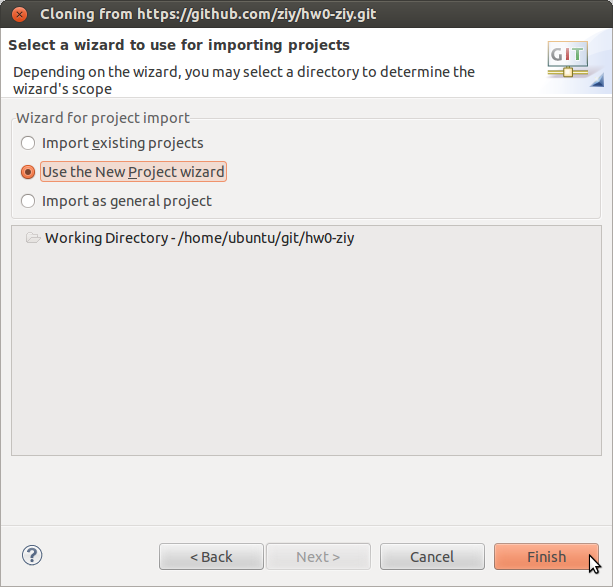
\includegraphics[scale=0.3]{project-08-new-project}
\caption{Creating new project\label{project-08-new-project}}
\end{minipage}
\hfill
\begin{minipage}{0.5\textwidth}
\centering
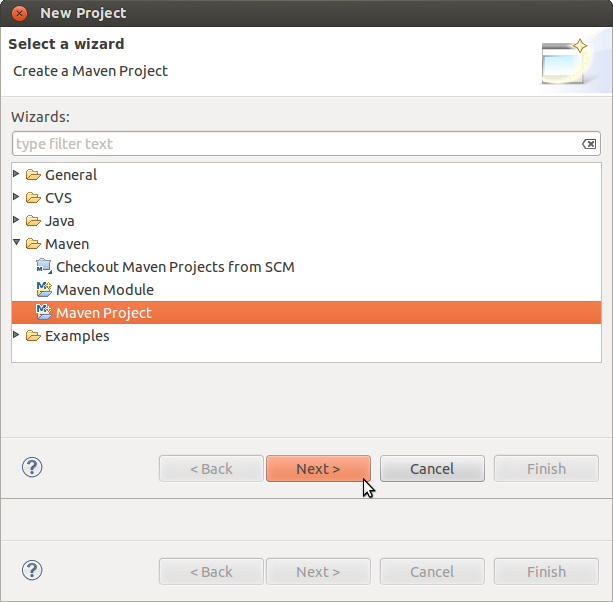
\includegraphics[scale=0.3]{project-09-maven}
\caption{Choosing to create new Maven project\label{project-09-maven}}
\end{minipage}
\hspace{-2em}
\end{figure}

\item Now, we select \textbf{Use the New Project wizard} in the ``Project
Import'' window and click \textbf{Finish} to begin create an Eclipse Maven
Project, as you can see in Figure \ref{project-08-new-project}.

\item Then select \textbf{Maven} $\rightarrow$ \textbf{Maven Project}, then
click \textbf{Next} to continue. See Figure \ref{project-09-maven}.

\begin{figure}[t]
\hspace{-3em}
\begin{minipage}{0.5\textwidth}
\centering
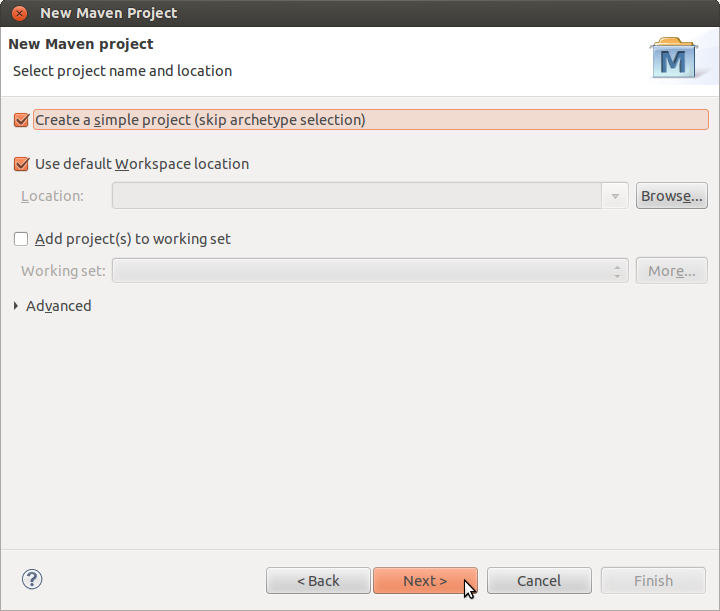
\includegraphics[scale=0.3]{project-10-maven-location}
\caption{Specifying Maven Project location\label{project-10-maven-location}}
\end{minipage}
\hfill
\begin{minipage}{0.5\textwidth}
\centering
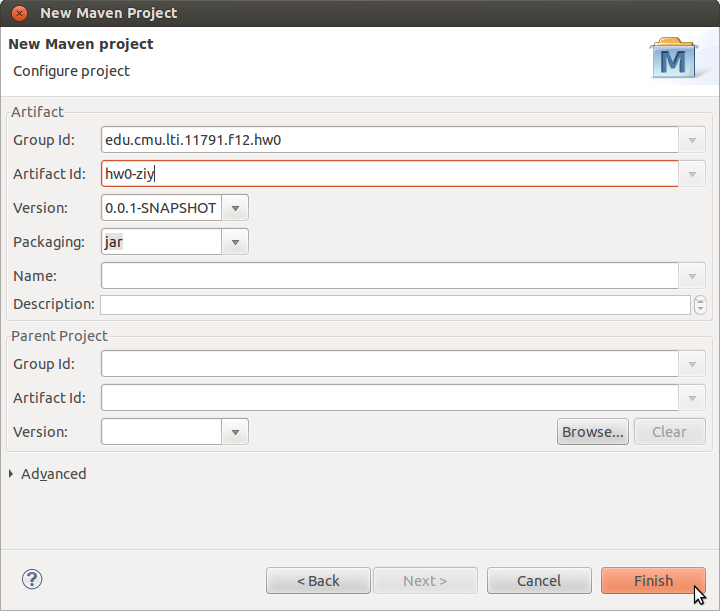
\includegraphics[scale=0.3]{project-11-maven-artifact}
\caption{Typing in basic information for Maven artifact\label{project-11-maven-artifact}}
\end{minipage}
\hspace{-3em}
\end{figure}

\item In the ``New Maven Project'' window, you select both \textbf{Create a
simple project (skip archetype selection)} and \textbf{Use default Workspace
location}. See Figure \ref{project-10-maven-location}. If you have already
forgotten what archetype and artifact are, you really need to go back to Task 1
to review the basic concepts of Maven. For Homework 0, you will not need an
archetype to base on, but you will soon realize that Maven archetypes are
crucial to software development. We will provide you the archetype you need for
Homework 1 and 2 (of course, via our course Maven repository).

\item Then, in the next window, you need to type in the \textbf{Group Id} and
\textbf{Artifact Id} for the artifact you are going to create. The Group Id for
Homework 0 is

\begin{center}
\textbf{edu.cmu.lti.11791.f14.hw0}
\end{center}

and the Artifact Id should be

\begin{center}
\textbf{hw0-ANDREW\_ID}
\end{center}

Replace \textbf{ANDREW\_ID} with your Andrew ID. You must type in the correct
information to create your artifact, since both Group Id and Artifact Id will be
used to generate the jar file and eventually submit the jar to the correct
folder in our Maven repository. You do not need to change the rest of the
configuration, and press \textbf{Finish} to complete creating the Maven project.
On some platforms\footnote{For example, Windows XP/Helios as reported by Martin
van Velsen}, you will need to fill in a Name and Description otherwise the
wizard will generate an error.

\begin{figure}[t]
\centering
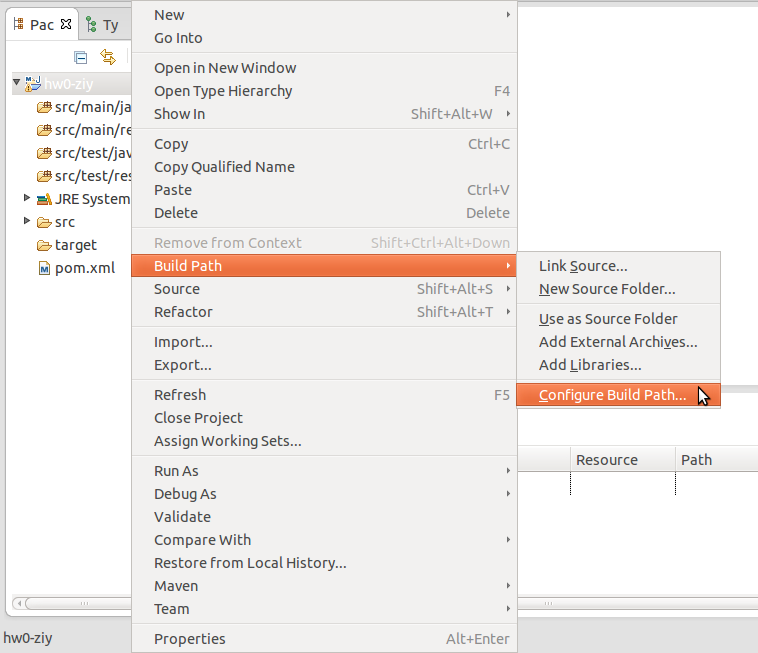
\includegraphics[scale=0.3]{project-12-jre}
\caption{Configuring Build Path\label{project-12-jre}}
\end{figure}

\item If you find the project is built based on an earlier version of Java
(e.g., JDK 1.5), then it is time to change it to JDK 6. If JDK environment that
your project is using is 1.6, then you can skip this additional step. First,
right-click on the project name (i.e. hw0-ziy) in the ``Package Explorer'' view,
which is usually located on the left of your workspace. Then select
\textbf{Build Path} $\rightarrow$ \textbf{Configure Build Path\ldots}, as shown
in Figure \ref{project-12-jre}.

\begin{figure}[t]
\centering
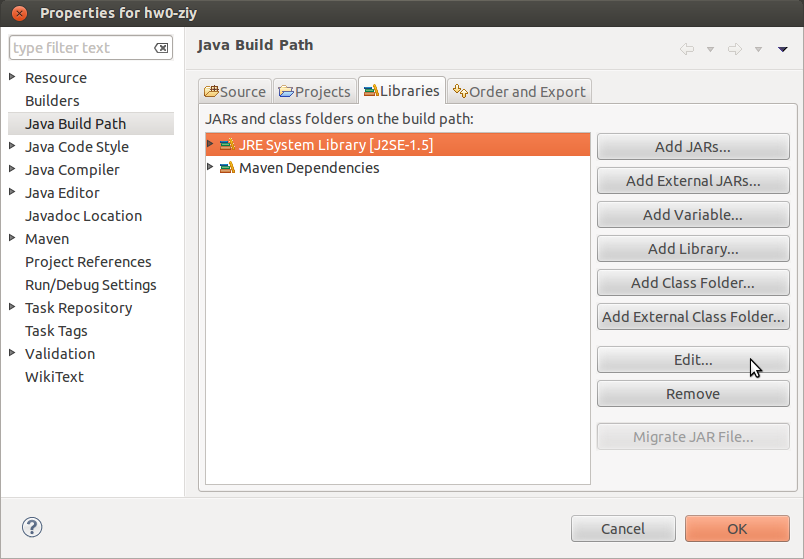
\includegraphics[scale=0.3]{project-13-jre-view}
\caption{Viewing JRE version\label{project-13-jre-view}}
\end{figure}

\item Then click the \textbf{Libraries} tab, select \textbf{JRE System Library},
and click \textbf{Edit}. See Figure \ref{project-13-jre-view}.

\begin{figure}[t]
\centering
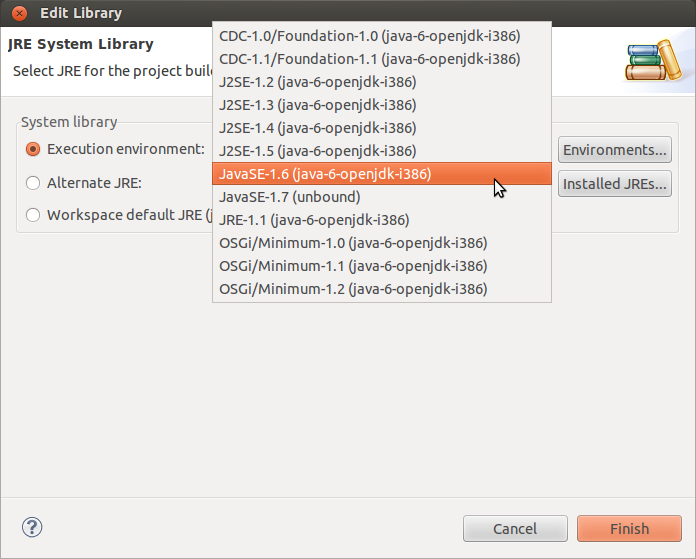
\includegraphics[scale=0.3]{project-14-jre-change}
\caption{Choosing a different JRE version\label{project-14-jre-change}}
\end{figure}

\item In the popup window, select any Jave 1.6 environment you have installed.
Note that the options in your workspace might be totally different from what you
see in Figure \ref{project-14-jre-change}.

\end{enumerate}

\subsection{Sharing your project via Git}

If you encountered the problem we described in Figure \ref{project-05-git-empty}
and \ref{project-06-git-local}, you need to re-establish the connection from the
local Git repository to the repository you built on GitHub. If you do not have
such issue, you can skip this part.

\begin{figure}[t]
\centering
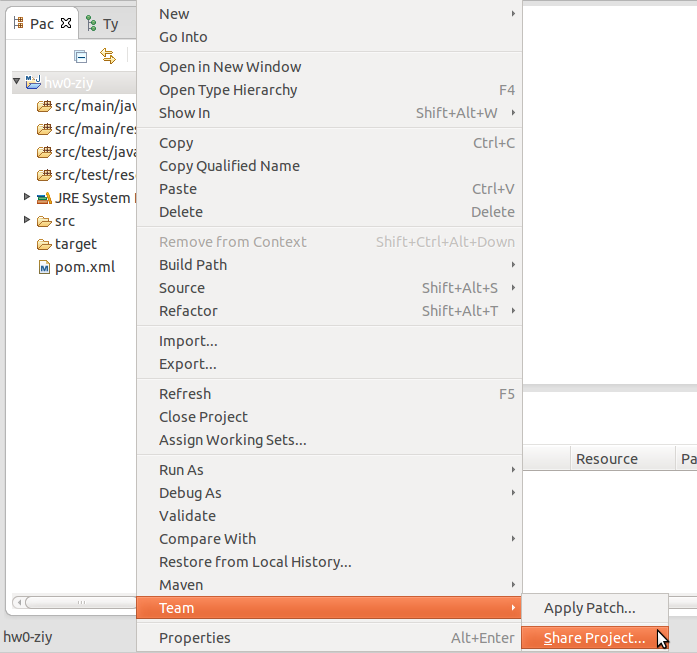
\includegraphics[scale=0.3]{project-15-share}
\caption{Sharing project again\label{project-15-share}}
\end{figure}

You need to right-click on the project name, and select \textbf{Team}
$\rightarrow$ \textbf{Share Project\ldots} in order to share your project on
GitHub. See Figure \ref{project-15-share}. You should be able to proceed by
selecting the repository type (Git). If you still find come across the NO-HEAD
issue (see Figure \ref{project-18-git-nohead}) after you share your project,
don't panic as you can specify the branch during your first git-commit.

\begin{figure}[t]
\centering
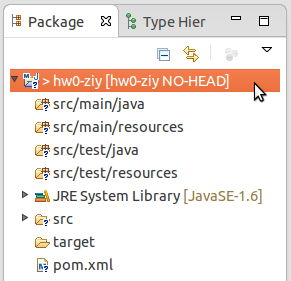
\includegraphics[scale=0.3]{project-18-git-nohead}
\caption{Nohead issue\label{project-18-git-nohead}}
\end{figure}

